\section{Motivation}
JavaScript Object Notation (JSON) is a human and machine-readable representation for text data.  It is widely used because of its simple and concise structure.  For example, Twitter uses  JSON as the only supported format for exchange of data starting from API v1.1 \cite{twitter-api}, and YouTube  recommends uses of JSON for speed from its latest API.  JSON  is being adapted increasingly in  large and scalable document databases such as MongoDB \cite{mongodb}, Apache Casandra \cite{cassandra} and CouchDB \cite{couchdb}. Besides  these, JSON is also widely used in lightweight data storages for example in configuration files, online catalogs or  applications with embedded storage.


%For the high adoption of these document databases,  recently, OpenStack  Database service, Trove, provides support for MongoDB starting from  Icehouse release \cite{openstack-support-mongodb}

In spite of high adoption from industry, JSON has received little attention from academic researchers. To the best of our knowledge, there is no formal work published  on the protection of JSON documents.


On the other hand, considerable work has been done for protection of XML documents. Although syntactically JSON and XML formats are different, semantically both of them form a rooted tree hierarchical structure. In fact, JSON data can equivalently be represented in XML form and vice versa. This brings an obvious question---whether we can utilize  authorization models used for XML documents for protection of  JSON data?


% 
 	\begin{figure} 
 		\centering
 		\includegraphics[width=.9\textwidth]{example-json-data}
 		\caption{Example of JSON Data}
 		\label{fig:example-json-data}
 	\end{figure}
 

Before we answer the preceding question, we look into some of the salient characteristics of data represented in JSON (or XML) format, given below.  

%In Figure \ref{fig:example-json-data} (a) we present employee records in a flat JSON file. The same records has been re-organized and presented in Figure \ref{fig:example-json-data} (b).  We believe, the key characteristics of JSON data to be considered for specification of authorization policies are as follows.

\begin{itemize}
	
	\item \textbf{Hierarchical relationship.} Data often exhibits hierarchical relationship. For example, a residential address consists of pieces like house number, street name, district/town and state name organized into a strictly hierarchical structure. 
	
	
	\item \textbf{Semantical association.} Different pieces of data are often related semantically and may need same level of protection.  For example, phone number, email address, Skype name may all represent contact information and require same level of protection.
	
	\item \textbf{Scatteredness.} Related information can be scattered around a document. For example, different pieces of contact information might be located in different places in a document. Some pieces of data can even be repeated in more than one place in the same document or across documents.  
	
	%For example, \ref{fig:example-json-data} (b), \textit{email} and \textit{work-phone} is placed under both \textit{public-info} and \textit{contact-info}.
\end{itemize}




Interestingly, most XML authorization models \cite{policy-based4,policy-based2,policy-based5,policy-based6} consider \textit{structural hierarchy} only. These models have an implicit assumption that information has been organized in the intended hierarchical form. These models attach authorization policies directly on nodes in the XML tree  and propagate them using the hierarchical structure. For example, Damiani et al. \cite{damiani2002fine} specify authorization policy as a tuple $\langle subject, object, action,$ $sign, type \rangle$ where subject is specified as user, user group, IP address or semantic name;  object is specified with XPath expression; example of actions are read or  write; signs are positive and negative; and example of types are local, global and DTD (Document Type Definition) which determines the level of propagation.  In this model, if similar data items requiring same level of protection are placed in structurally unrelated nodes, it is required to attach same authorization policy to all these nodes. This results in duplication of authorization policies which is caused by lack of recognition of semantical association and scatteredness properties. 

%Propagation of authorization policies in these model is solely based on structural hierarchy. As a result, these models suffer in the maintenance of authorization policies. 

Duplication incurs significant overhead in maintenance of authorization policies. For instance, if requirements for storing or publishing contact information (e.g. email, phone, fax) change, it is required to update policies for all different pieces of data that represent contact information. Organizations often collect different types of data including personal identifiable information of employees and customers. So, they need to comply to different internal and external requirements including from government and standard bodies. This increases the likelihood that authorization requirements change frequently over time. 

% This also increases the possibility of  inconsistencies due to unintended mistakes. 


%\textbf{Duplicated authorization policies.} If an XML element appear in more than one nodes (for example, in Figure \ref{fig:example-json-data} \textit{email} appears in two different node), we need to duplicate the same authorization policies in each node. While we need to update authorization policies, we need to update all duplicated policies. Assuming policy update is not infrequent, this poses significant maintenance overhead. 

While most XML authorization models directly identify nodes in their authorization policies, our proposed model adds a level of abstraction by using \textit{security-label} attribute values. The proposed model specifies two types of policies, called \textit{authorization policies} and \textit{labeling policies}.  Authorization policies are specified using \textit{security-label} attribute values. These values are assigned to JSON data using labeling policies. A conceptual overview of existing XML authorization models and our proposed model is  shown schematically in Figures \ref{fig:indirection}(a) and \ref{fig:indirection}(b) respectively. By using security-label attribute values to connect nodes and policies, we can assign to same attribute-values to semantically related or scattered data. This eliminates the need to specify duplicated policies.
	
 
 	\begin{figure} [t]
 		\centering
 		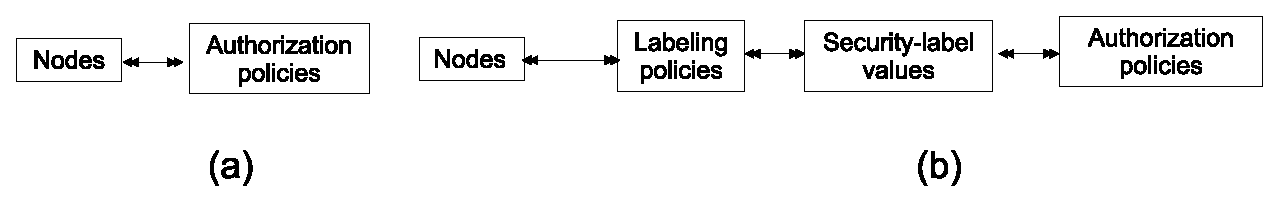
\includegraphics[width=.9\textwidth]{NSS16/indirection}
 		\caption{Synopsis of (a) existing XML models  and, (b) the proposed model}
 		\label{fig:indirection}
 	\end{figure}
 
	
%In this paper, we propose attribute based specification of authorization policies for protecting JSON document. Though we consider JSON data, the same protection model can also be used for XML documents as well. We consider one user attribute called \textit{user-label} or  \textit{uLabel} in short and one object attribute called \textit{security-label} or \textit{sLabel} in short. \textit{uLabel} values are assigned on users and \textit{sLabel} values are assigned on JSON elements. For each authorization action, we specify one policy consisting of enumerated micro-policies using these labels.  For example, the authorization policy $Auth_{read}$= \textit{\{(HR, contact-info)\}} specify that all users who are assigned value \textit{HR} can read all JSON objects which are assigned value \textit{contact-info}. Our protection model is adapted from the enumerated ABAC model\cite{labac}. 






The proposed model additionally offers flexibility in specification and maintenance of  authorization and labeling policies. These two types of policies can now be managed separately and independently. For instance, given \textit{security-label} attribute values, higher level, organization-wide policy makers can specify authorization policies using these values without knowing details of JSON structure. On the other hand, local administrators knowledgeable about details of specific JSON documents can specify labeling policies. 


The presented model can easily be generalized for data represented in trees and be instantiated for other representations, for example, YAML. For simplicity, we only focus on JSON here.